\documentclass{easytikz}

\begin{document}
  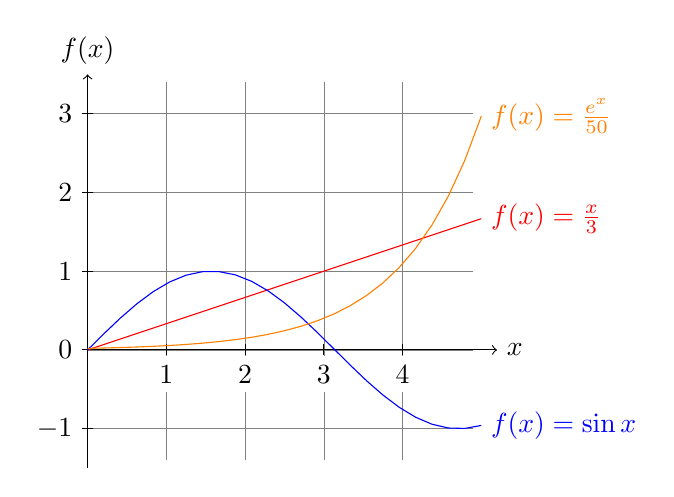
\begin{tikzpicture}[domain=0:5]
    \draw[very thin,gray] (0,-1.4) grid (4.9,3.4);
    \draw[->] (0,0) -- (5.2,0) node[right] {$x$};
    \draw[->] (0,-1.5) -- (0,3.5) node[above] {$f(x)$};
    %
    \foreach \x in {1,...,4}
      \draw[xshift=\x cm] (0,2pt) -- (0,-2pt) node[below,fill=white] {$\x$};
    \foreach \y in {-1,...,3}
      \draw[yshift=\y cm] (2pt,0) -- (-2pt,0) node[left,fill=white] {$\y$};
    %
    \draw[red]    plot (\x,\x/3)         node[right] {$f(x) = \frac{x}{3}$};
    \draw[blue]   plot (\x,{sin(\x r)})  node[right] {$f(x) = \sin x$};
    \draw[orange] plot (\x,{exp(\x)/50}) node[right] {$f(x) = \frac{e^x}{50}$};
  \end{tikzpicture}
\end{document}